\begin{figure}[t]
	\centering
	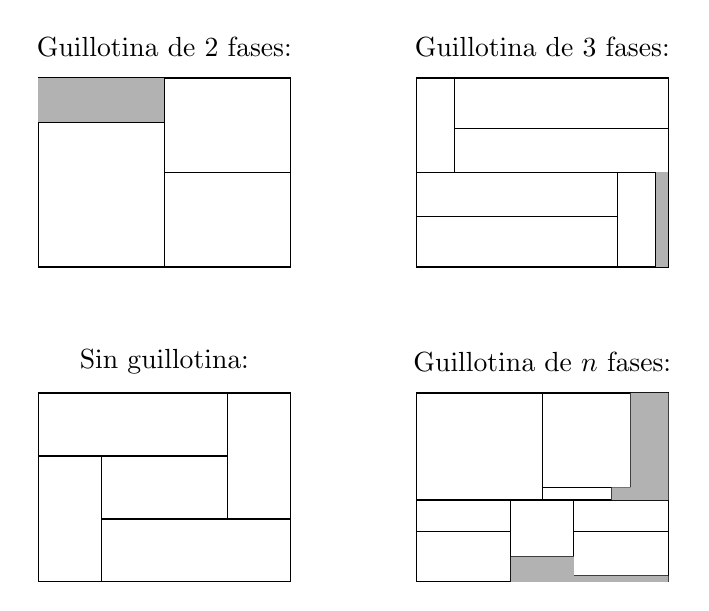
\begin{tikzpicture}[scale = 0.80]
		% sin guillotina:
		\node at (2,3.5) {Sin guillotina:};
		\draw (0, 0) -- (4, 0) -- (4, 3) -- (0, 3) -- cycle ;
		\draw (0, 2) -- (3, 2);
		\draw (1, 0) -- (1, 2);
		\draw (1, 1) -- (4, 1);
		\draw (3, 1) -- (3, 3);

		% n-guillotina:
		\node at (8,3.5) {Guillotina de $n$ fases:};
		\draw (6, 0) -- (10, 0) -- (10, 3) -- (6, 3) -- cycle;
		\draw (6, 1.3) -- (10, 1.3);
		\draw (7.5, 0) -- (7.5, 1.3);
		\draw (8.5, 0) -- (8.5, 1.3);
		\draw (8, 1.3) -- (8, 3);
		\draw (6, 0.8) -- (7.5, 0.8);
		\draw (8.5, 0.8) -- (10, 0.8);
		\draw (8.5, 0.1) -- (10, 0.1);
		\draw (7.5, 0.4) -- (8.5, 0.4);
		\draw (7.5, 0.4) -- (8.5, 0.4);
		\draw (8, 1.5) -- (10, 1.5);
		\draw (9.4, 1.5) -- (9.4, 3);
		\draw (9.1, 1.5) -- (9.1, 1.3);
		\fill[gray!60]  (7.5, 0) -- (7.5, 0.4) -- (8.5, 0.4) -- 
						(8.5, 0.1) -- (10, 0.1) -- (10, 0) -- cycle;
		\fill[gray!60]  (9.4, 3) -- (10, 3) -- (10, 1.3) -- (9.1 ,1.3) --
						(9.1, 1.5) -- (9.4, 1.5) -- cycle;

		% 2- guillotina:
		\node at (2,8.5) {Guillotina de 2 fases:};
		\draw (0, 5) -- (4, 5) -- (4, 8) -- (0, 8) -- cycle ;
		\draw (2, 5) -- (2, 8);
		\draw (2, 6.5) -- (4, 6.5);
		\draw (0, 7.3) -- (2, 7.3);
		\fill[gray!60] (0, 8) -- (0, 7.3) -- (2, 7.3) -- (2, 8) -- cycle;

		% 3- guillotina:
		\node at (8,8.5) {Guillotina de 3 fases:};
		\draw (6, 5) -- (10, 5) -- (10, 8) -- (6, 8) -- cycle ;
		\draw (6, 6.5) -- (10, 6.5);
		\draw (6.6, 7.2) -- (10, 7.2);
		\draw (6.6, 8) -- (6.6, 6.5);
		\draw (6, 5.8) -- (9.2, 5.8);
		\draw (9.2, 5) -- (9.2, 6.5);
		\draw (9.8, 5) -- (9.8, 6.5);
		\fill[gray!60] (9.8, 5) -- (9.8, 6.5) -- (10, 6.5) -- (10, 5) -- cycle;
	\end{tikzpicture}
	\caption{Ejemplo de patrones para cortes con guillotina.}
	\label{fig:patrones}
\end{figure}
